\documentclass[../main.tex]{subfiles}
\begin{document}


\subsection{Creazione Macchina}
Come prima cosa bisognerà aprire virtual box e cliccare in alto a destra sul tasto \textbf{Nuova} una volta fatto ci si aprira la seguente schermata. In questa schermata andrà scelto il nome della macchina, dove salvare e in fine che sistema operativo vogliamo installare. 

\begin{figure}[h]
    \centering
    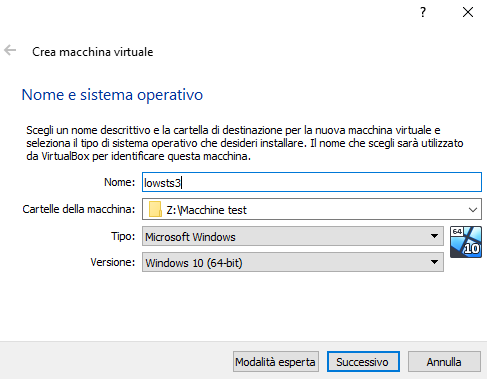
\includegraphics[width=0.6\textwidth]{Images/set-up1.PNG}
    \caption{Nome macchina}
\end{figure}
  Una votla fatto questo ci basterà cliccare su \textbf{Successivo} per andare avanti con l'installazione. E verremo portati alla schermata seguent.
  
\

\begin{figure}[h]
    \centering
    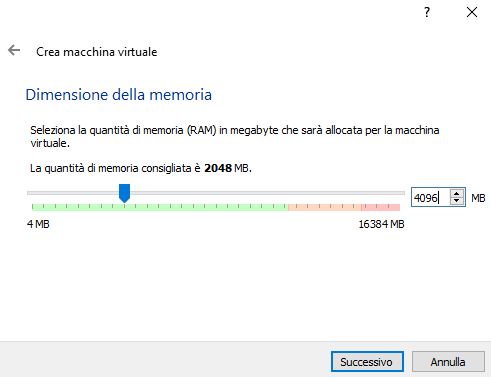
\includegraphics[width=0.6\textwidth]{Images/set-up2.PNG}
    \caption{Assegnazione RAM}
\end{figure}

\pagebreak{}
\thispagestyle{header-pages}

Una votla arrivati in questa schermata dovremmo solo impostare la ram in questo caso avendo a disposizione una macchina con 16 GB di RAM ho deciso di dare 4 GB di RAM a questa macchina virtuale. Anche qui una volta imessa quanta RAM vogliamo ci basterÀ cliccare successivo e procedere.

\textbf{Remember la quantità di RAM che assegni deve essere 1024 moltipilicato quanta ram vuoi dare nel mio caso 4GB di RAM quindi 1024*4}

Per le prossime due schermata ci basterà andare avanti. Fino a arrivare alla schermata seguente

\begin{figure}[h]
    \centering
    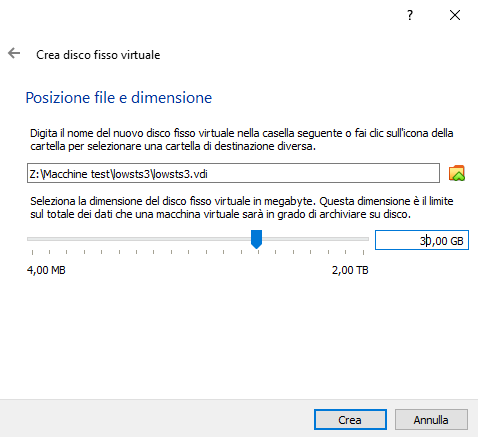
\includegraphics[width=0.5\textwidth]{Images/set-up5.PNG}
    \caption{Assegnazione spazio al disco}
\end{figure}


In questa schermata dovremmo insteire quanta memoria vorrrmo che la nostra macchina virtuale abbia in questo caso scriviamo 30,00 GB e cliccare il tasto \textbf{Crea}.


\begin{figure}[h]
    \centering
    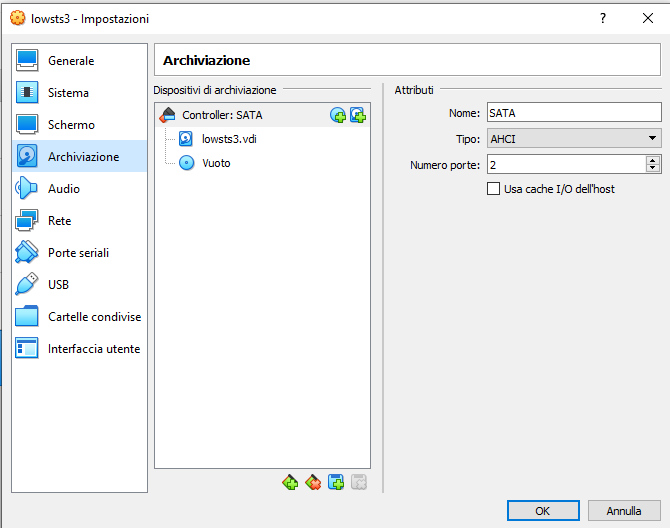
\includegraphics[width=0.5\textwidth]{Images/set-up6.PNG}
    \caption{Aggiunta dell'ISO}
\end{figure}
\pagebreak{}
\thispagestyle{header-pages}

Una volta fatto tutto questo ci manca solo l'ultima cosa cioè collegare la iso alla nostra macchina virtuale. Ci bastera cliccare sul disco vuoto e cliccare aggiungi e selezionare la nostra iso.



Una volta avviata la macchina virtuale partirà questa schermata ci basterà cliaccare \textbf{avanti} e poi \textbf{installa}. 
\begin{figure}[h]
    \centering
    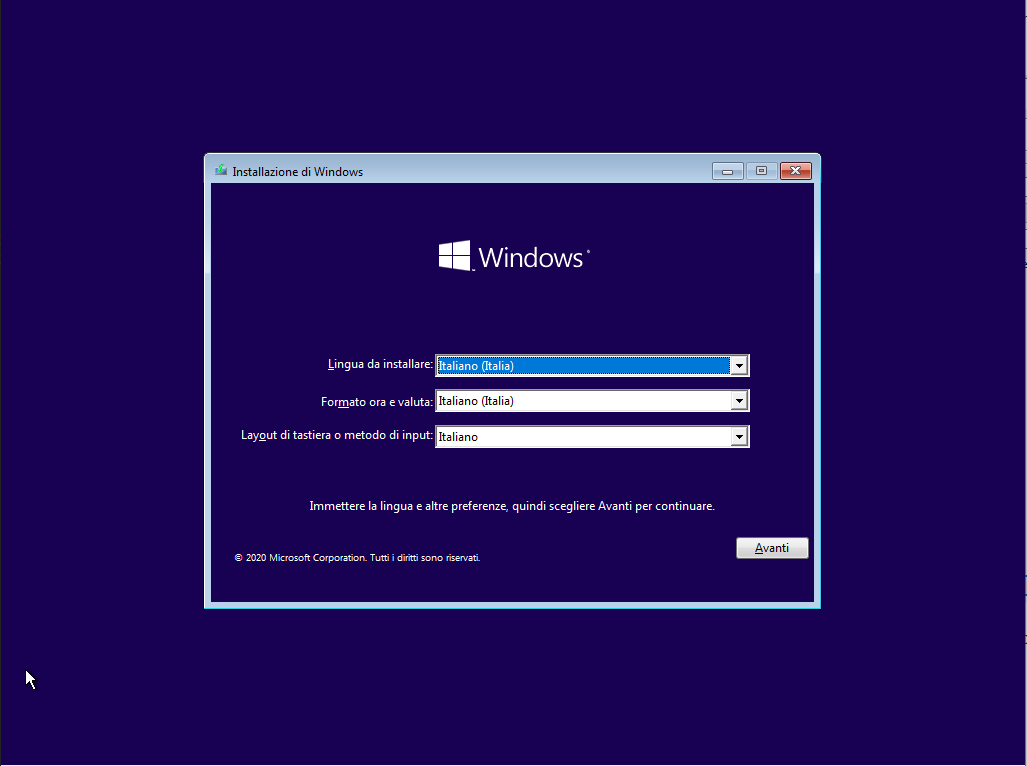
\includegraphics[width=0.75\textwidth]{Images/conf1.PNG}
    \caption{Scelta lingua}
\end{figure}
Una volta arrivati in questa schermata dovremmo cliccare su \textbf{Non ho un codice Produt Key} e ci caricherà una schermata dove ci chiederà che versione di Windows vorremmo installare. Vedi foto seguente.


\begin{figure}[h]
  \centering
  \begin{minipage}[h]{0.45\textwidth}
    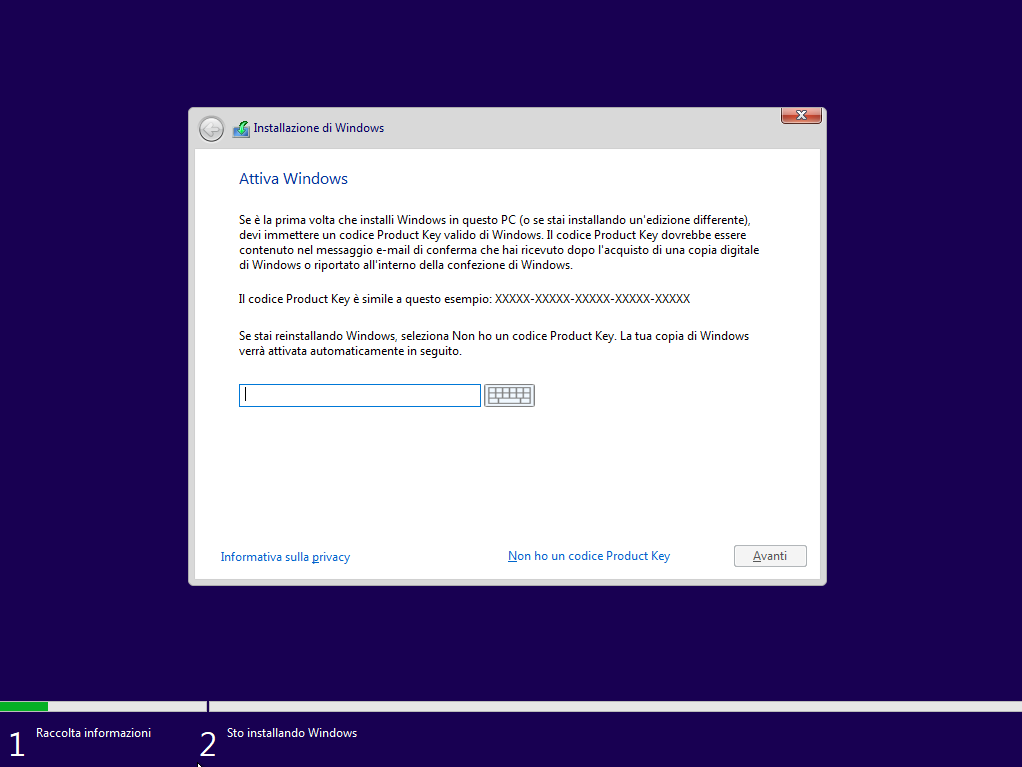
\includegraphics[width=\textwidth]{Images/conf2.PNG}
    \caption{Produt Key}
  \end{minipage}
  \hfill
  \begin{minipage}[h]{0.45\textwidth}
    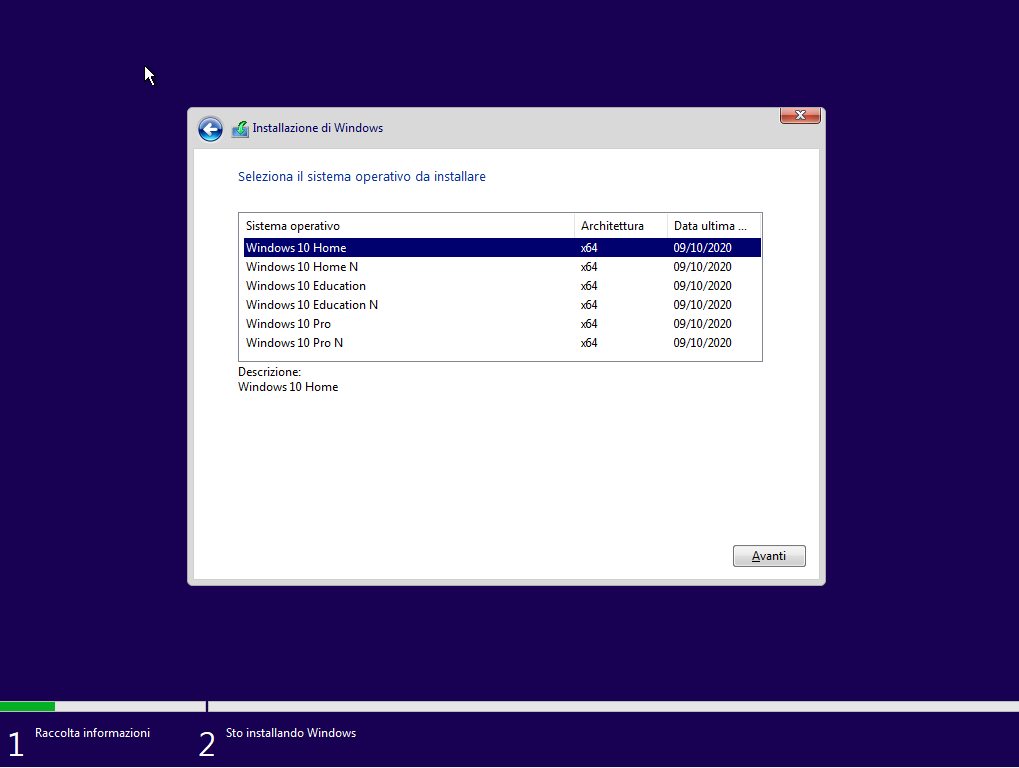
\includegraphics[width=\textwidth]{Images/conf3.PNG}
    \caption{Scelta della versione}
  \end{minipage}
\end{figure}



Qui ci basterà cliccare la versione nel nostro caso Windows  10 education e cliccare su \textbf{avanti}.Dopo di che ci chiederà di accettare i termini della licienza bisgona accettare e andare avanti. Ci caricherà una schermata dove che tipo di installazione si vuole eseguire. Noi sceglieremo Quella personalizzata, ci verrà chiesto su che disco la vogliamo installare e ci mostrerà solo un disco. Quindi senza fare niente ci basterà cliccare su \textbf{avanti}. Dopo aver cliccato avanti partirà l'installazione. 


\end{document}  
